%! TEX program = lualatex

% Use :VimtexToggleMain to compile this file alone with Vimtex
\documentclass[tikz]{standalone}

\usepackage{sty/adantikz}

\begin{document}
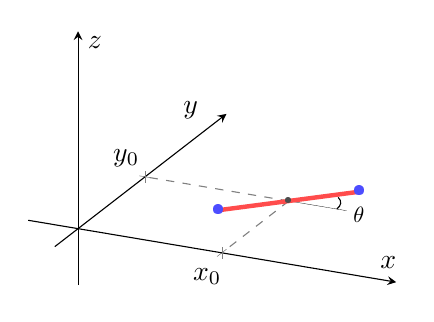
\begin{tikzpicture}[x={(8.66cm,5cm)},y={(0cm,10cm)},z={(8.66cm,-5cm)}]
\begin{axis}[
axis on top,
axis lines = center,
% Set the size of the axes
xmin = -1, xmax = 15,
ymin = -1, ymax = 15,
zmin = -1, zmax = 5,
% Show the axis labels
xlabel = $x$,
ylabel = $y$,
zlabel = $z$,
% Make the tick marks more visible
enlargelimits = 0.1,
xtick = {7.5},
xticklabels={$x_0$},
ytick = {7.5},
yticklabels={$y_0$},
ztick = {0},
zticklabels={$ $},
% Shift the y labels to the other side
yticklabel style = {xshift={(-0.4cm)},yshift={(0.5cm)}},
]
% Set our coordinates 
\coordinate (p1) at (5,5,0);
\coordinate (p2) at (10,10,0);
\coordinate (com) at (7.5,7.5,0);
% Draw theta
\draw[draw=black, ultra thin] (com) -- (10.5,7.5,0) 
	node[above,scale=0.8,xshift=0.2cm,yshift=-0.3cm]{$\theta$};
\draw (10,7.5,0) arc (0:45:2);
% Draw the dashed lines for the x and y axes
\draw[draw=gray, dashed] (com) -- (7.5,0,0);
\draw[draw=gray, dashed] (com) -- (0,7.5,0);
% Draw the bar and COM
\draw[draw=red!70,ultra thick] (p1) -- (p2); 
\node[scale=0.6] at (com) {\textcolor{black!70}{\textbullet}};

% Draw the first point
\node at (p1) {\textcolor{blue!70}{\textbullet}};
% Draw the second point
\node at (p2) {\textcolor{blue!70}{\textbullet}};
\end{axis}
\end{tikzpicture}
\end{document}
% vim: set tw=80 ts=4 sw=4 sts=0 et ffs=unix :
